\documentclass[tikz,border=8pt]{standalone}
\usepackage[T1]{fontenc}
\usepackage{helvet}
\renewcommand{\familydefault}{\sfdefault}
\usetikzlibrary{arrows.meta,positioning,fit,backgrounds,calc}
\pagecolor{white}

% colorblind-safe palette (Okabe-Ito)
\definecolor{cOrange}{HTML}{D55E00}
\definecolor{cBlue}{HTML}{0072B2}
\definecolor{cGreen}{HTML}{009E73}
\definecolor{cGrey}{HTML}{555555}
\definecolor{cOrangeBg}{HTML}{FBEDE3}
\definecolor{cBlueBg}{HTML}{E3EEF6}
\definecolor{cGreenBg}{HTML}{E2F3EE}
\definecolor{cGreyBg}{HTML}{F2F2F2}

\begin{document}
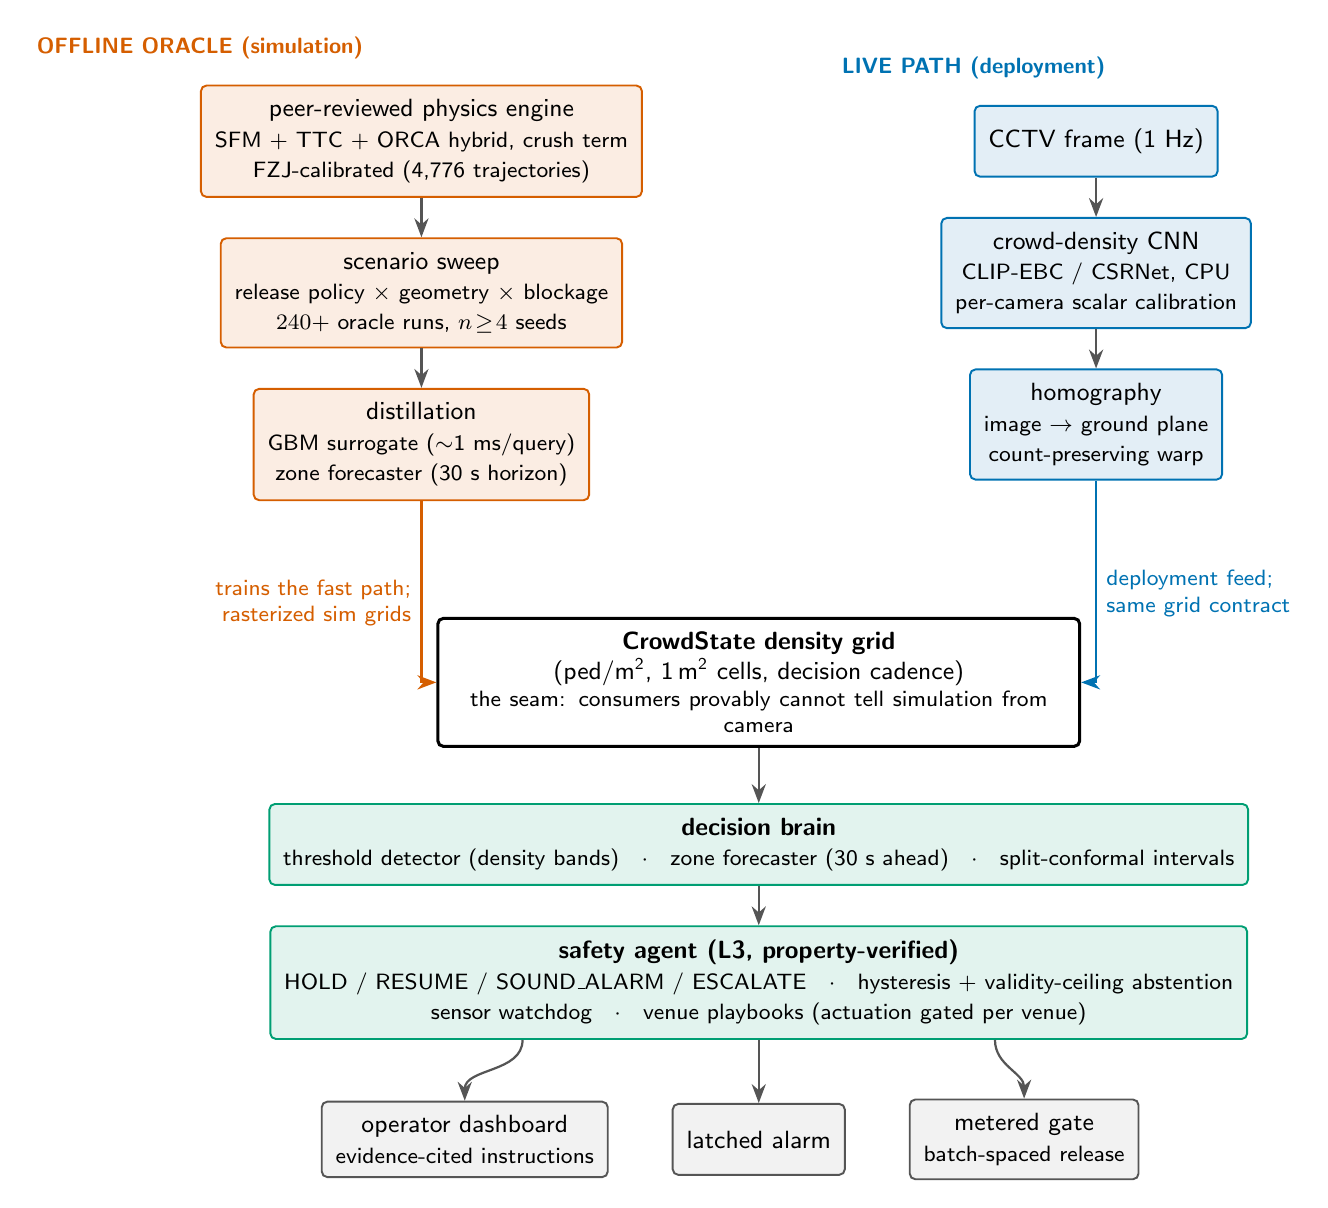
\begin{tikzpicture}[
  font=\small,
  node distance=5mm and 8mm,
  box/.style={draw, rounded corners=2pt, align=center, inner sep=5pt,
              minimum height=9mm, line width=0.7pt},
  offline/.style={box, draw=cOrange, fill=cOrangeBg},
  live/.style={box, draw=cBlue, fill=cBlueBg},
  brain/.style={box, draw=cGreen, fill=cGreenBg},
  sink/.style={box, draw=cGrey, fill=cGreyBg},
  arr/.style={-{Stealth[length=2.4mm]}, line width=0.8pt, cGrey},
  lane/.style={font=\footnotesize\bfseries, anchor=west},
]

% ---------- offline lane ----------
\node[offline] (engine) {peer-reviewed physics engine\\
  \footnotesize SFM + TTC + ORCA hybrid, crush term\\
  \footnotesize FZJ-calibrated (4{,}776 trajectories)};
\node[offline, below=of engine] (sweep) {scenario sweep\\
  \footnotesize release policy $\times$ geometry $\times$ blockage\\
  \footnotesize $240+$ oracle runs, $n\!\ge\!4$ seeds};
\node[offline, below=of sweep] (train) {distillation\\
  \footnotesize GBM surrogate ($\sim$1 ms/query)\\
  \footnotesize zone forecaster (30 s horizon)};

% ---------- live lane ----------
\node[live, right=42mm of engine] (cam) {CCTV frame (1 Hz)};
\node[live, below=of cam] (cnn) {crowd-density CNN\\
  \footnotesize CLIP-EBC / CSRNet, CPU\\
  \footnotesize per-camera scalar calibration};
\node[live, below=of cnn] (homog) {homography\\
  \footnotesize image $\to$ ground plane\\
  \footnotesize count-preserving warp};

% ---------- the seam ----------
\path (train.south) -- (homog.south) coordinate[midway] (mid);
\node[box, draw=black, fill=white, line width=1.1pt, below=16mm of mid,
      text width=78mm] (seam)
  {\centering\textbf{CrowdState density grid}\\
   (ped/m\textsuperscript{2}, 1\,m\textsuperscript{2} cells, decision cadence)\\
   \footnotesize the seam: consumers provably cannot tell simulation from camera\par};

% ---------- brain ----------
\node[brain, below=7mm of seam] (detector)
  {\textbf{decision brain}\\
   \footnotesize threshold detector (density bands) \; $\cdot$ \;
   zone forecaster (30 s ahead) \; $\cdot$ \; split-conformal intervals};
\node[brain, below=of detector] (agent)
  {\textbf{safety agent (L3, property-verified)}\\
   \footnotesize HOLD / RESUME / SOUND\_ALARM / ESCALATE \; $\cdot$ \;
   hysteresis + validity-ceiling abstention\\
   \footnotesize sensor watchdog \; $\cdot$ \; venue playbooks (actuation gated per venue)};

% ---------- outputs ----------
\node[sink, below=8mm of agent] (alarm) {latched alarm};
\node[sink, left=8mm of alarm] (dash) {operator dashboard\\ \footnotesize evidence-cited instructions};
\node[sink, right=8mm of alarm] (gate) {metered gate\\ \footnotesize batch-spaced release};

% ---------- arrows ----------
\draw[arr] (engine) -- (sweep);
\draw[arr] (sweep) -- (train);
\draw[arr] (cam) -- (cnn);
\draw[arr] (cnn) -- (homog);
\draw[arr, cOrange] (train.south) |- (seam.west)
  node[pos=0.28, left, font=\footnotesize, text=cOrange, align=right]
  {trains the fast path;\\rasterized sim grids};
\draw[arr, cBlue] (homog.south) |- (seam.east)
  node[pos=0.28, right, font=\footnotesize, text=cBlue, align=left]
  {deployment feed;\\same grid contract};
\draw[arr] (seam) -- (detector);
\draw[arr] (detector) -- (agent);
\draw[arr] (agent.south) -- (alarm.north);
\draw[arr] ($(agent.south)+(-30mm,0)$) to[out=-90,in=90] (dash.north);
\draw[arr] ($(agent.south)+(30mm,0)$) to[out=-90,in=90] (gate.north);

% ---------- lane labels ----------
\node[lane, text=cOrange, above=2mm of engine.north west] {OFFLINE ORACLE (simulation)};
\node[lane, text=cBlue, above=2mm of cam.north west] {LIVE PATH (deployment)};

\end{tikzpicture}
\end{document}
